\documentclass[12pt,a4paper,utf8]{ctexart}
\usepackage{graphicx}
\usepackage{amsmath}
\usepackage{amssymb}
\usepackage{subfig}
\usepackage{cite}
\usepackage[ntheorem]{empheq}
\usepackage{enumitem}
\usepackage{fullpage}
\usepackage{cleveref}
\usepackage{cellspace}
\usepackage{listings}
\usepackage{color}
\usepackage[top=2cm, bottom=2cm, left=2cm, right=2cm]{geometry}  
\usepackage{algorithm}  
\usepackage{algorithmicx}  
\usepackage{algpseudocode}  
\renewcommand{\algorithmicrequire}{\textbf{Input:}}  % Use Input in the format of Algorithm  
\renewcommand{\algorithmicensure}{\textbf{Output:}} % Use Output in the format of Algorithm 
\definecolor{gray}{rgb}{0.5,0.5,0.5}
\definecolor{dkgreen}{rgb}{.068,.578,.068}
\definecolor{dkpurple}{rgb}{.320,.064,.680}

% set Matlab styles
\lstset{
   language=Matlab,
   keywords={break,case,catch,continue,else,elseif,end,for,function,
      global,if,otherwise,persistent,return,switch,try,while},
   basicstyle=\small\ttfamily,
   keywordstyle=\color{blue}\bfseries,
   commentstyle=\color{dkgreen},
   stringstyle=\color{dkpurple},
   backgroundcolor=\color{white},
   tabsize=4,
   showspaces=false,
   showstringspaces=false
}

\begin{document}
\CJKfamily{zhkai}	


\begin{center}
\textbf{作业一}\\
\textbf{姓名:晏瑞然~~~~~~~~~~~~~ 学号:PB19000196~~~~~~~~~~~~~~ 日期:4.28}\\
\end{center}

\begin{center}
\fbox{
\begin{minipage}{40em}
\vspace{5cm}
\hspace{20cm}
\end{minipage}}
\end{center}
\vspace{1cm}

\begin{enumerate}
\item[第一题] \textbf{线性系统求解}  

(a),(b):

两题中生成图如下,由图可知$\omega=1.6$时收敛速度最快。

\begin{figure}[h]
   \centering
   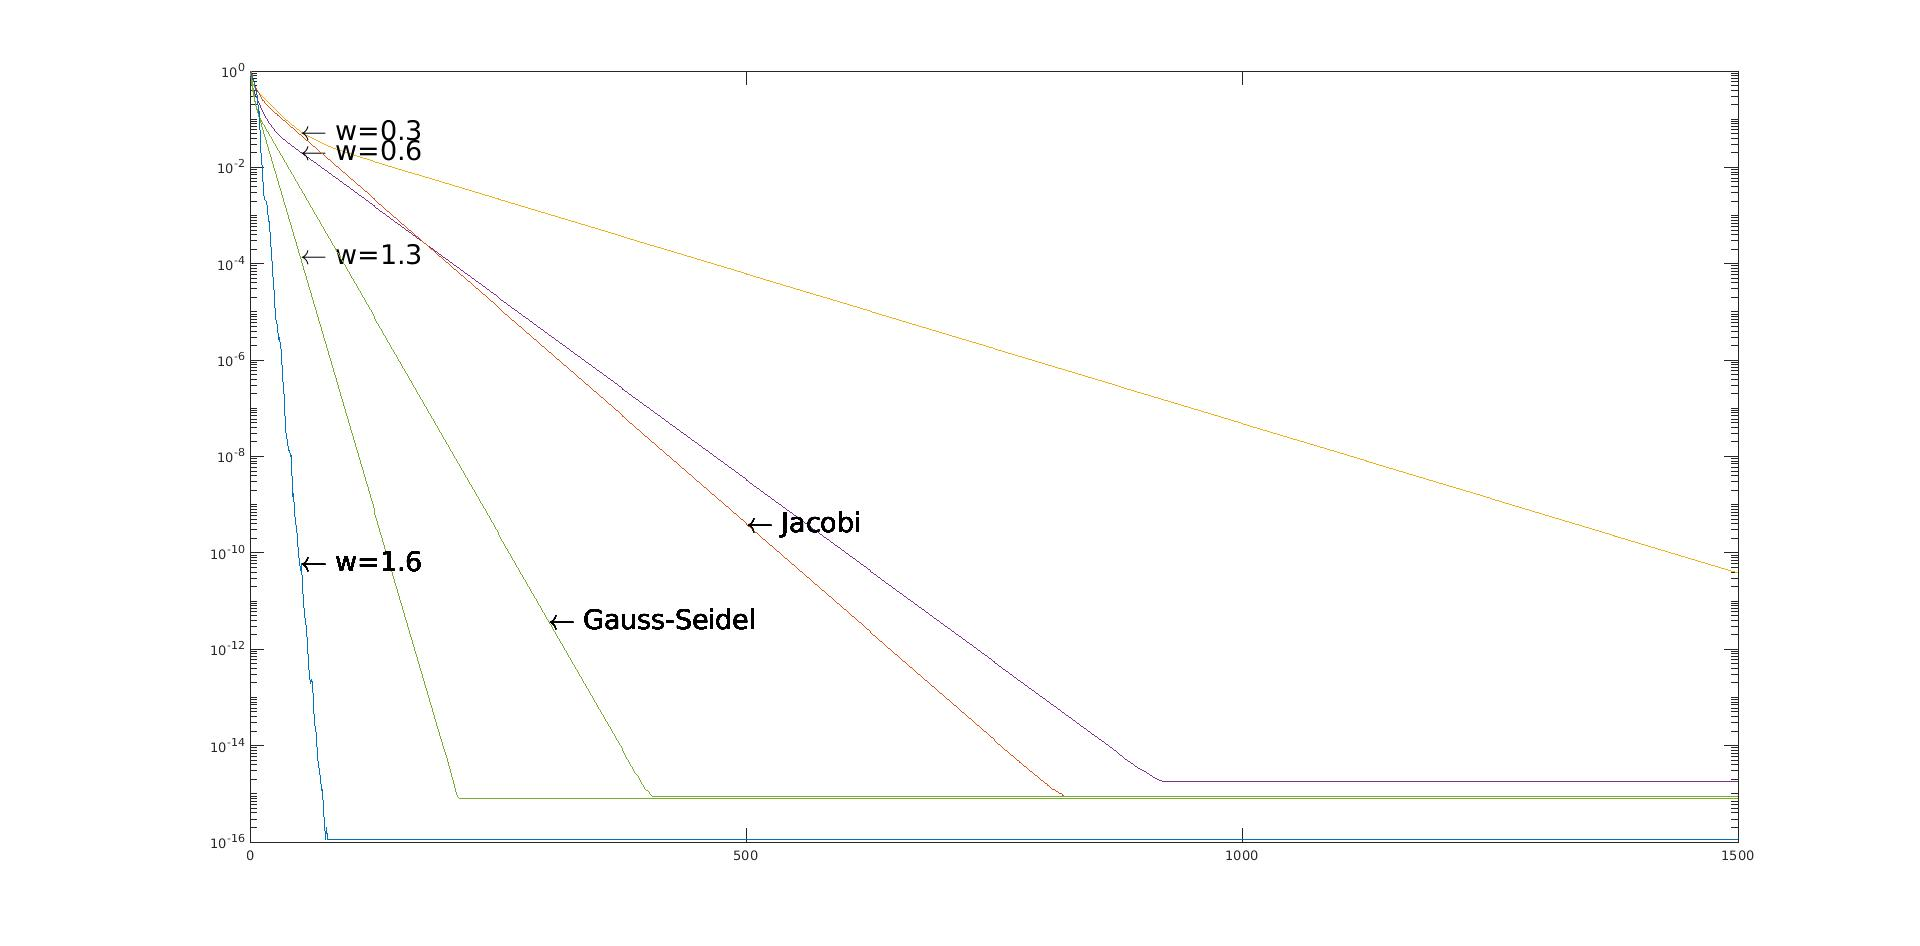
\includegraphics[width=15cm,height=8cm]{ex1_2.jpg}
   \caption{第一题(a)、(b)}
\end{figure}

(c):
程序思路:
不使用矩阵运算,直接将每次迭代用循环表达。
这样可以避免0元素的运算。

程序说明:
因为单次运算时间过短,每次统计计算10次运算的结果,除去第一次统计,统计10-1次。
实验中限制迭代次数为1500次,SOR迭代中$\omega=1.6$,所得时间单位为秒,保留4位小数。

实验数据如下:

\begin{table}[h]

   \caption{实验数据表(除去第一次)}
	\begin{tabular}{ | c | c | c | c | c | c | c | c | c | c |}
		\hline
		实验次数 	            & 2 & 3 & 4 & 5 & 6 & 7 & 8 & 9 & 10 \\ 
		\hline
		Jacobi(未加速) 	      & 0.0079 & 0.0048 & 0.0061 & 0.0050 & 0.0076 & 0.0056 & 0.0053 & 0.0055 & 0.0049 \\ 
		\hline 
		Jacobi(加速)            & 0.0040 & 0.0038 & 0.0041 & 0.0038 & 0.0041 & 0.0038 & 0.0040 & 0.0039 & 0.0041 \\ 
		\hline 
      Gauss(未加速) 	         & 0.0500 & 0.0315 & 0.0399 & 0.0351 & 0.0436 & 0.0427 & 0.0345 & 0.0361 & 0.0333 \\ 
		\hline 
		Gauss(加速)             & 0.0022 & 0.0022 & 0.0022 & 0.0021 & 0.0021 & 0.0020 & 0.0021 & 0.0021 & 0.0021 \\ 
		\hline 
      SOR(未加速)  	         & 0.0323 & 0.0297 & 0.0321 & 0.0344 & 0.0367 & 0.0283 & 0.0409 & 0.0294 & 0.0308 \\ 
		\hline 
		SOR(加速)               & 0.0026 & 0.0026 & 0.0029 & 0.0032 & 0.0027 & 0.0025 & 0.0025 & 0.0025 & 0.0026 \\ 
		\hline 
	\end{tabular}
\end{table}

统计平均结果如下:
\begin{table}[h]
   \centering
   \caption{统计平均结果}
	\begin{tabular}{ | c | c | c |}
		\hline
			            & 未加速 	& 加速	 \\ 
		\hline
		Jacobi 	      & 0.0059	& 0.0040		 \\ 
		\hline 
		Gauss-Seidel   & 0.0354 & 0.0021		 \\ 
      \hline 
		SOR            & 0.0327 & 0.0027		 \\
		\hline 
	\end{tabular}
\end{table}

MATLAB程序如下:

主函数:
\begin{lstlisting}[frame=single]
% ex1.a.b
aaa = ones(10,1);
bbb = [-aaa,aaa*2,-aaa];
A = spdiags(bbb,[-1 0 1],10,10);
b = [2;-2;2;-1;0;0;1;-2;2;-2];
x_exact = [1;0;1;0;0;0;0;-1;0;-1];
timeList = zeros(3,2);
% J method
J(A,b,x_exact);
% G method
G(A,b,x_exact);
w=[0.3 0.6 1.3 1.6];
for i=1:4
    S(A,b,x_exact,w(i));
end

%ex1.c
%迭代次数:1500,Sor迭代w=1.6
T=zeros(10,1);
for i =1:10
    [~,T(i)]=J(A,b,x_exact);
end
timeList(1,1) = sum(T)-T(1);
for i =1:10
    [~,T(i)]=G(A,b,x_exact);
end
timeList(2,1) = sum(T)-T(1);
for i =1:10
    [~,T(i)]=S(A,b,x_exact,1.6);
end
timeList(3,1) = sum(T)-T(1);
for i =1:10
    [~,T(i)]=J2(A,b,x_exact);
end
timeList(1,2) = sum(T)-T(1);
for i =1:10
    [~,T(i)]=G2(A,b,x_exact);
end
timeList(2,2) = sum(T)-T(1);
for i =1:10
    [~,T(i)]=S2(A,b,x_exact,1.6);
end
timeList(3,2) = sum(T)-T(1);
timeList
\end{lstlisting}
各子函数:
\begin{lstlisting}[frame=single]
function [x,time] = J(A,b,x_exact)
%J 使用Jacobi迭代求解线性系统,不加速

% 对角矩阵的逆可以由对角线上元素取倒数得到
D_inverse = diag(diag(1./A));
R = eye(size(A)) - D_inverse*A;
g = D_inverse*b;
err = zeros(1500,1);
x = eye(size(b));
tic
for i=1:1500
   err(i) = max(abs(x-x_exact));
   x = R*x+g;
end
time = toc;
a = 1:1500;
semilogy(a,err)
s = '\leftarrow Jacobi';
text(500,err(500),s,'FontSize',20)
hold on
end
\end{lstlisting}

\begin{lstlisting}[frame=single]
function [x2,time] = J2(A,b,x_exact)
%J2 使用Jacobi迭代求解线性系统,加速

D = diag(A);
D_inv = 1./D;
err = zeros(1500,1);
x2 = eye(size(b));
xsize=size(b,1);
tic
for i=1:1500
   x1 = x2;
   err(i)=max(abs(x2-x_exact));
   x2(1)=D_inv(1)*(b(1)+x1(2));
   for j=(1+1):(size(b,1)-1)
      x2(j)=D_inv(j)*(b(j)+x1(j-1)+x1(j+1));
   end
   x2(xsize) = D_inv(xsize)*(b(xsize)+x1(xsize-1));
end
time = toc;
err(1500);
end
\end{lstlisting}

\begin{lstlisting}[frame=single]
function [x,time] = G(A,b,x_exact)
%G 使用Gauss-Seidel迭代求解线性系统,不加速

D = diag(diag(A));
L = tril(A)-diag(diag(A));
U = triu(A) - diag(diag(A));
err = zeros(1500,1);
x = eye(size(b));
tic
for i=1:1500
      err(i) = max(abs(x-x_exact));
      x = (D+L)\(-U*x+b);
end
time = toc;
a = 1:1500;
semilogy(a,err)
s = '\leftarrow Gauss-Seidel';
text(300,err(300),s,'FontSize',20)
hold on
end
\end{lstlisting}

\begin{lstlisting}[frame=single]
function [x,time] = G2(A,b,x_exact)
%G2 使用Gauss-Seidel迭代求解线性系统,加速

D = diag(A);
D_inv = 1./D;
err = zeros(1500,1);
x = eye(size(b));
tic
for i=1:1500
   err(i)=max(abs(x-x_exact));
   x(1)=D_inv(1)*(b(1)+x(2));
   for j=(1+1):(size(b,1)-1)
      x(j)=D_inv(j)*(b(j)+x( j-1)+x(j+1));
   end
   x(size(b,1))=D_inv(size(b,1))*(b(size(b,1))+x(size(b,1)-1));
end
time = toc;
err(1500);
end
\end{lstlisting}

\begin{lstlisting}[frame=single]
function [x,time] = S(A,b,x_exact,w)
%S 使用Sor迭代求解线性系统,不加速

D = diag(diag(A));
L = tril(A)-diag(diag(A));
U = triu(A) - diag(diag(A));
D_inverse = diag(diag(1./A));
L_tilde = -D_inverse*L;
U_tilde = -D_inverse*U;
g = D_inverse*b;

err = zeros(1500,1);
x = eye(size(b));
tic
for i=1:1500
   err(i) = max(abs(x-x_exact));
   %if err(i)< 1e-15
   %    break;
   %end
   x = (eye(size(A))-w.*L_tilde)\...
   (((1-w).*eye(size(A))+w.*U_tilde)*x+w.*g); 
end
time = toc;

a = 1:1500;
semilogy(a,err)
s = ['\leftarrow w=',num2str(w)];
text(50,err(50),s,'FontSize',20)
hold on

end
\end{lstlisting}

\begin{lstlisting}[frame=single]
function [x,time] = S2(A,b,x_exact,w)
%S2 使用Sor迭代求解线性系统,加速

D = diag(A);
D_inv = 1./D;
err = zeros(1500,1);
x = eye(size(b));
xsize=size(b,1);
tic
for i=1:1500
   err(i)=max(abs(x-x_exact));
   x(1)=(1-w)*x(1)+w*D_inv(1)*(b(1)+x(2));
   for j=(1+1):(size(b,1)-1)
      x(j)=(1-w)*x(j)+w*D_inv(j)*(b(j)+x(j-1)+x(j+1));
   end
x(xsize) = (1-w)*x(xsize)+w*D_inv(xsize)* ...
(b(xsize)+x(xsize-1));
end
time = toc;
err(1500);
end
\end{lstlisting}

\item[第二题]\textbf{Newton法求解方程}

(a)、(b):

程序思路:
选取初始值$x_l=-1.5,x_m=0.5,x_r=3$,进行牛顿迭代。
在迭代过程中,每生成3个迭代值,用$x_{k+2}$代替精确解计算
$\log(|x_{k+1}-x_{k+2}|),\log(|x_{k+1}-x_{k+2}|)$,
再由每两组上述值计算斜率,即为迭代的阶数。

程序说明:
$x$为不同初始值得到的解。
$x(i)\_list$为上述解得到的迭代过程,i可以取$l,m,r$,分别代表三个解的迭代过程。
$n(i)$为得到上述迭代估算的阶的过程,其最后一个元素即为估算的阶。

程序结果:

程序结果如下,由结果可以看出三个解分别是
$x_l=-0.732,x_m=1,x_r=2.732$,
阶分别为$n_l=2,n_m=3,n_r=2$。

\begin{lstlisting}[frame=single]
   x =

   -0.732050807568877
 
 
 xl_list =
 
   -1.500000000000000
   -0.984126984126984
   -0.773163127830252
   -0.733437807950018
   -0.732052470495501
   -0.732050807571272
   -0.732050807568877
 
 
 nl =
 
    1.568545332745191
    1.856274573297303
    1.984324400495861
    1.999720993874996
 
 
 x =
 
      1
 
 
 xm_list =
 
    0.500000000000000
    1.111111111111111
    0.999074074074074
    1.000000000529222
    1.000000000000000
 
 
 nm =
 
    3.192460317189232
    3.002594709561758
 
 
 x =
 
    2.732050807568877
 
 
 xr_list =
 
    3.000000000000000
    2.777777777777778
    2.733756613756614
    2.732053321730378
    2.732050807574352
    2.732050807568877
 
 
 nr =
 
    1.845924079368328
    1.982116998528189
    1.999631420917110
\end{lstlisting}

(c):

确实出现了阶比2大的现象,出现原因如下:

Newton法对应于$f(x)=0$的迭代方程为$\varphi (x)=x-\frac{f(x)}{f'(x)}$。

对$\varphi (x)$求导得:

$\varphi' (x)=\frac{f(x)f''(x)}{(f'(x))^2}$

$\varphi'' (x)=\frac{(f'(x)f''(x)+f'''(x)f(x))f'(x)^2-2f'(x)f(x)f''(x)^2}{(f'(x))^4}$

...

设真实解为$\alpha$本题中$\alpha=1$,该解十分特殊,因为此解同时满足$f(\alpha)=0,f''(\alpha)=0$。
将$\alpha$带入$\varphi (x)$的各阶导数,得:

$\varphi (\alpha)=\alpha,\varphi' (\alpha)=0,\varphi'' (\alpha)=0,\varphi''' (\alpha)\neq 0$

故:

$\quad x_{k+1}-\alpha \\
= \varphi (x_k)-\varphi (\alpha)\\
=\varphi (\alpha)+(x_k-\alpha)\varphi' (\alpha)+\frac{(x_k-\alpha)^2}{2!}\varphi'' (\alpha)+\frac{(x_k-\alpha)^3}{3!}\varphi''' (\xi )-\varphi (\alpha) \\
=\frac{(x_k-\alpha)^3}{3!}\varphi''' (\xi )$

$\Rightarrow \lim_{k \to \infty} \frac{|x_{k+1}-\alpha |}{|x_k-\alpha |^3}=\frac{\varphi''' (\alpha)}{3!} $

此时,牛顿迭代的阶变为3阶。

MATLAB程序如下:
\begin{lstlisting}[frame=single]
format long
xl0=-1.5;
xm0=0.5;
xr0=3;
a0=[1,-3,0,2];
a1=[3,-6,0];
m=10;%迭代次数
err=[];
xl_list=xl0;
x=xl0;
nl=[];
for i=1:m
   x1=x-(a0(1)*x^3+a0(2)*x^2+a0(3)*x+a0(4)) ... 
   /(a1(1)*x^2+a1(2)*x+a1(3));
   if abs(x1-x)<=1e-15
      break
   end
   err=[err;(x1-x)];
   if i>2
      loge_k_0=log10(abs(err(i-2)+err(i-1)));
      loge_k_1=log10(abs(err(i-1)+err(i)));
      loge_kplus1_0=log10(abs(err(i-1)));
      loge_kplus1_1=log10(abs(err(i)));
      nl=[nl;(loge_kplus1_0-loge_kplus1_1)/(loge_k_0-loge_k_1)];
   end
   xl_list = [xl_list;x1];
   x=x1;
end
x
xl_list
%err;
nl
err=[];
xm_list=xm0;
x=xm0;
nm=[];
for i=1:m
   x1=x-(a0(1)*x^3+a0(2)*x^2+a0(3)*x+a0(4)) ... 
   /(a1(1)*x^2+a1(2)*x+a1(3));
   if abs(x1-x)<=1e-15
      break
   end
   err=[err;(x1-x)];
   if i>2
      loge_k_0=log10(abs(err(i-2)+err(i-1)));
      loge_k_1=log10(abs(err(i-1)+err(i)));
      loge_kplus1_0=log10(abs(err(i-1)));
      loge_kplus1_1=log10(abs(err(i)));
      nm=[nm;(loge_kplus1_0-loge_kplus1_1)/(loge_k_0-loge_k_1)];
   end
   xm_list = [xm_list;x1];
   x=x1;
end
x
xm_list
%err;
nm
err=[];
xr_list=xr0;
x=xr0;
nr=[];
for i=1:m
   x1=x-(a0(1)*x^3+a0(2)*x^2+a0(3)*x+a0(4)) ... 
   /(a1(1)*x^2+a1(2)*x+a1(3));
   if abs(x1-x)<=1e-15
      break
   end
   err=[err;(x1-x)];
   if i>2
      loge_k_0=log10(abs(err(i-2)+err(i-1)));
      loge_k_1=log10(abs(err(i-1)+err(i)));
      loge_kplus1_0=log10(abs(err(i-1)));
      loge_kplus1_1=log10(abs(err(i)));
      nr=[nr;(loge_kplus1_0-loge_kplus1_1)/(loge_k_0-loge_k_1)];
   end
   xr_list = [xr_list;x1];
   x=x1;
end
x
xr_list
%err;
nr
\end{lstlisting}

\newpage
\item[第三题]\textbf{幂法求特征值}  

(a):
\begin{algorithm}[htbp] 
   \caption{幂法求最大特征值}  
   \begin{algorithmic}[1] 
      \Require
      A: 待求特征值矩阵;  
      X: 迭代初始值;  
      $\epsilon$: 最大误差;
      itr: 迭代次数; 
    \Ensure  
      $\lambda$: A的模最大特征值;
      $v$: $\lambda$对应的特征向量;
     \For{each $i\in [1,itr]$}  
       \State $Y^{(k)}=X^{(k)}/\left\lVert X^{(k)}\right\rVert _{\infty }$;  
       \State $X^{(k+1)}=AY^{(k)}$;  
     \EndFor  
     \If {$max_{1\leq i\leq n}|\frac{x_i^{(k+1)}}{y_i^{(k)}}-\frac{x_i^{(k)}}{y_i^{(k-1)}}|<\epsilon$} 
       \State $\lambda =\frac{x_i^{(k+1)}}{y_i^{(k)}},1\leq i\leq n$;
       \State $v=Y^{(k)}$
     \ElsIf {$max_{1\leq i\leq n}|\frac{Ax_i^{(k+1)}}{y_i^{(k)}}-\frac{Ax_i^{(k)}}{y_i^{(k-1)}}|<\epsilon$}
       \State $\lambda_1=\sqrt{\frac{Ax_i^{(k)}}{y_i^{(k-1)}}},1\leq i\leq n$
       \State $\lambda_2=-\lambda_1$
       \State $v_1=AX^{(k+1)}+\lambda_1 X^{(k)}$
       \State $v_2=AX^{(k+1)}-\lambda_1 X^{(k)}$
     \EndIf
   \end{algorithmic}  
 \end{algorithm}  

(b):

设$A1=A,A2=-A$,由程序得:
\begin{lstlisting}[frame=single]

\end{lstlisting}

MATLAB程序如下:


\begin{lstlisting}[frame=single]

\end{lstlisting}

\end{enumerate}




\end{document}
